\section{HyperBRDF - Additional Results}
\label{hyperbrdf:add_res}

\subsection{Full Reconstruction}\label{sec:full_rec}

We first evaluated the full reconstruction capacity of our method by using all available samples during the inference time. Figure \ref{fig:qual_comp} shows our results without/with LRM (Sec. \ref{sec:lrm}) along with the results for Hyper autoencoder (Hyper-AE) \cite{sztrajman2021neural}, PCA, and IPCA. For all methods, we do the same train/test split and compare the methods both qualitatively (Figure \ref{fig:qual_comp}) and quantitatively (Table \ref{table: comparison results}) over the test set. Please note that Hyper-AE is not included in the results for reconstruction with sparse samples since it only works with a fixed grid of input samples, unable to reconstruct materials with varying sizes. 


Figure \ref{fig:qual_comp} shows that our method attains superior results in terms of the reconstruction quality of measured BRDFs. The reconstructed materials with PCA or Hyper-AE cannot capture the material properties, such as the diffuse components, effectively. They can also cause some artifacts (chrome, green-metallic-paint). The linear structure of PCA cannot handle the high dynamic range of the data. Although IPCA \cite{nielsen2015optimal} improves the results substantially, they still have difficulty capturing the right colors. The NBRDF \cite{sztrajman2021neural} reconstruction results can be found in their supplementary. Since our hypernetwork model offers a generalizable approach to NBRDF, it is expected that an overfitting NBRDF model performs better in reconstruction with full samples. 

\begin{figure*}
  \centering
\adjustbox{trim={0.\width} {.\height} {0.\width} {.\height},clip}%
  {\includegraphics[width=0.66\linewidth]{Chapters/hyperbrdf-figs/qualitative_comp_40_all_samples.pdf}}
    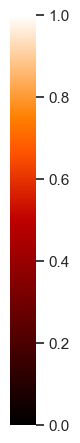
\includegraphics[width=0.02\linewidth]{Chapters/hyperbrdf-figs/vbar.png}

   \caption{Qualitative comparison for full reconstruction capacity on the test dataset.}
    % \RM{Why you are not comparing with GGX?}

   \label{fig:qual_comp}
\end{figure*}

\begin{table*}
    \centering
    \caption{Quantitative comparison results for full reconstruction over the renderings of the test set.}
        \resizebox{0.9\linewidth}{!}
    {\begin{tabular}{l@{\hskip 0.2in}c@{\hskip 0.2in}c@{\hskip 0.2in}c@{\hskip 0.2in}c@{\hskip 0.2in}c}\toprule
 & Hyper-AE & PCA &  IPCA & Ours (No LRM) & Ours \\
\toprule
 PSNR \textuparrow & 21.696 & 16.407 & 28.471 & 20.696 & \cellcolor{blue!25}33.128 \\
  Delta E \textdownarrow & 7.761 & 13.233 & 4.023 & 8.970 & \cellcolor{blue!25}2.181 \\
 SSIM\textuparrow & 0.873 & 0.818 & 0.975 & 0.896 & \cellcolor{blue!25}0.978 \\
 MAE\textdownarrow & 13.058 & 30.949 & 5.940 & 16.927 & \cellcolor{blue!25}3.574 \\
 RMSE\textdownarrow & 23.051 & 47.018 & 10.276 & 28.314 & \cellcolor{blue!25}6.740 \\
 RAE\textdownarrow & 0.329 & 0.780 & 0.158 & 0.421 & \cellcolor{blue!25}0.091 \\

\bottomrule
    \end{tabular}\par}
    \label{table: comparison results}

\end{table*}

\subsection{Compression}
We report the rendering results of 100 MERL materials for compression (Table \ref{table: oursvsnps}):
% \begin{figure*}
%   \centering
%  \includepdf[pages=-]{Chapters/hyperbrdf-figs/comp-crop.pdf}

%  % {\includegraphics[width=\linewidth]{Chapters/hyperbrdf-figs/Compression.pdf}}
%     % \RM{Why you are not comparing with GGX?}

%    \label{fig:full-comp}
% \end{figure*}

%\begin{table}
 %   \centering
   % \caption{GGX - Average metric results over the renderings of our test dataset. We highlight \colorbox{blue!25}{best} results.}

    {%
    %{\begin{tabular}{l@{\hskip 0.3in}c@{\hskip 0.1in}c@{\hskip 0.1in}c@{\hskip 0.1in}c@{\hskip 0.1in}c@{\hskip 0.1in}c}\toprule


  %$N$ &  PSNR \textuparrow & Delta E \textdownarrow & SSIM \textuparrow & MAE \textdownarrow  & RMSE \textdownarrow & RAE \textdownarrow\\ 
 %\toprule
 %$40$ & 29.198 & 2.821 & 0.924 & 6.724 &  12.778 & 0.141\\
 %$160$ &28.893 & 2.831 &  0.923 &6.906 & 13.004 & 0.147\\
% $400$ & 29.193 & 2.771 & 0.924 &  6.722 & 12.798 & 0.141\\
 %$2000$ &  29.040 & 2.794 & 0.923 & 6.795 & 12.919 & 0.143\\
 %$4000$ & 29.035 & 2.792 & 0.923 & 6.786 & 12.914 & 0.143\\
 %All samples & \cellcolor{blue!25} 30.334 & \cellcolor{blue!25}2.241 & \cellcolor{blue!25}0.967 & \cellcolor{blue!25}4.784 & \cellcolor{blue!25}8.787 & \cellcolor{blue!25}0.123\\
%\bottomrule
  %  \end{tabular}\par}}
    %\label{tab:ggx}
%\end{table}



% \clearpage
\begin{figure*}
  \centering
  % \fbox{\rule{0pt}{2in} \rule{0.9\linewidth}{0pt}}
   % \includegraphics[width=\linewidth]{fig/different_sample_result_ext.pdf}

  {\includegraphics[width=0.72\linewidth]{Chapters/hyperbrdf-figs/supp_40.pdf}}
      % {\includegraphics[width=0.45\linewidth]{Chapters/hyperbrdf-figs/supp_40_rms.pdf}}
  {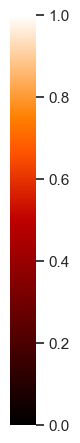
\includegraphics[width=0.02\linewidth]{Chapters/hyperbrdf-figs/vbar.png}}
   \caption{Sparse reconstruction results, $N = 40$.}
   \label{fig:40}
\end{figure*}

% \clearpage
\begin{figure*}
  \centering
  % \fbox{\rule{0pt}{2in} \rule{0.9\linewidth}{0pt}}
   % \includegraphics[width=\linewidth]{fig/different_sample_result_ext.pdf}

  {\includegraphics[width=0.72\linewidth]{Chapters/hyperbrdf-figs/supp_160.pdf}}
      % {\includegraphics[width=0.45\linewidth]{Chapters/hyperbrdf-figs/supp_160_rms.pdf}}
  {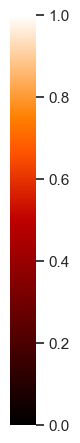
\includegraphics[width=0.02\linewidth]{Chapters/hyperbrdf-figs/vbar.png}}
   \caption{Sparse reconstruction results, $N = 160$.}
   \label{fig:160}
\end{figure*}

% \clearpage
\begin{figure*}
  \centering
  % \fbox{\rule{0pt}{2in} \rule{0.9\linewidth}{0pt}}
   % \includegraphics[width=\linewidth]{fig/different_sample_result_ext.pdf}

  {\includegraphics[width=0.72\linewidth]{Chapters/hyperbrdf-figs/supp_400.pdf}}
      % {\includegraphics[width=0.45\linewidth]{Chapters/hyperbrdf-figs/supp_400_rms.pdf}}
  {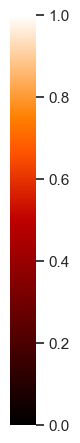
\includegraphics[width=0.02\linewidth]{Chapters/hyperbrdf-figs/vbar.png}}
   \caption{Sparse reconstruction results, $N = 400$.}
   \label{fig:400}
\end{figure*}

% \clearpage
\begin{figure*}
  \centering
  % \fbox{\rule{0pt}{2in} \rule{0.9\linewidth}{0pt}}
   % \includegraphics[width=\linewidth]{fig/different_sample_result_ext.pdf}

  {\includegraphics[width=0.72\linewidth]{Chapters/hyperbrdf-figs/supp_2000.pdf}}
      % {\includegraphics[width=0.45\linewidth]{Chapters/hyperbrdf-figs/supp_2000_rms.pdf}}
  {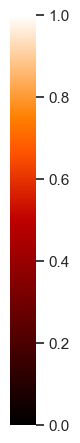
\includegraphics[width=0.02\linewidth]{Chapters/hyperbrdf-figs/vbar.png}}
   \caption{Sparse reconstruction results, $N = 2000$.}
   \label{fig:2000}
\end{figure*}

\begin{figure*}
  \centering
  % \fbox{\rule{0pt}{2in} \rule{0.9\linewidth}{0pt}}
   % \includegraphics[width=\linewidth]{fig/different_sample_result_ext.pdf}

  {\includegraphics[width=0.72\linewidth]{Chapters/hyperbrdf-figs/supp_4000.pdf}}
    % {\includegraphics[width=0.45\linewidth]{Chapters/hyperbrdf-figs/supp_4000_rms.pdf}}
  {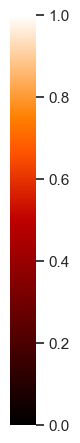
\includegraphics[width=0.02\linewidth]{Chapters/hyperbrdf-figs/vbar.png}}
   \caption{Sparse reconstruction results, $N = 4000$.}
   \label{fig:4000}
\end{figure*}


